\begin{comment}
\section{Memory Management}
Most programming languages uses stack and heap memory to organize the memory consumption of an application. Heap memory is used especially for dynamic allocated objects. During call stack unwinding, all the memory allocated in each frame is deleted there by automatically deleting unwanted memory in the frame. The idea of heap memory is also to enhance the life of the data. So a call stack unwinding does not delete all the memory allocated in the frame when it is popped. So this creates the necessity for developers to identify when the data has to be deleted and reclaim memory for reuse. 

Although memory management is broader term, in the context of this thesis, it refers to managing heap memory. There are two solutions to memory management. First, being manual memory management where the developers has to identify the life of the data / object and delete them. Another possibility, is to run a automated program that identifies all the unwanted data and delete them. The later is usually referred as automatic memory management or garbage collection. Programming languages that include garbage collection program in their runtime systems are referred as managed runtime systems. Managed runtime systems like JVM include a wide range of garbage collection programs to efficiently manage heap memory.

Data residing in the heap memory is only accesible by the pointers in the stack memory and static memory. These pointers are also called as roots. 

\end{comment}

\section{Abstract Graph Model}
\paragraph{Basic Reference Graph:}
We model the relationship among various objects and references in memory through a directed graph $G = (V, E)$, which we call a {\it reference graph}.
The graph $G$ has a special node $R$, which we call the {\it root}. Node $R$
represents
global and stack pointer variables, and
thus does not have any incoming edges.
Each node in $G$ is assumed to contain a unique ID. % to distinguish it within
%$G$. (For example, when each node of $G$ maps to a unique site in $H$, then ID of the site in $H$ can be used for the ID of the node in $G$.)
All adjacent nodes to a given node in $G$ are called $neighbors$, and denoted by $\Gamma$. The
$\inneighbors$ of a node $x\in G$ can be defined as the set of nodes whose outgoing edges
are incident on $x$, represented by $\Gamma_{in}(x)$. The $\outneighbors$ of $x$ can be defined as the set
of nodes whose incoming edges originate on $x$, represented by $\Gamma_{out}(x)$.
Note that each node $x\in G$ does not know $\Gamma_{in}(x)$ at any point in time.
%This constraint
%reduces memory complexity, thereby making
%the algorithm more practical and scalable. \todo{remove preceding sentence?}

\paragraph{Garbage Collection Problem:}
All nodes in $G$ can be classified as either {\em live} (i.e., not garbage) or {\em dead} (i.e., garbage) based on a property called
$reachability$. Live and dead nodes can be defined as below:


%$Live(x)= \exists y \in V \mid Reachable(y, x)$

%$Reachable(y, x) = x \in R \vee (Live(y) \wedge x \in \Gamma_{out}(y))$

$Reachable(y,x) = x \in \Gamma_{\rm out}(y) \lor (x \in \Gamma_{\rm out}(z) \mid Reachable(y,z))$

$Live(x) = Reachable(R,x)$

$Dead(x) = \neg Live(x)$

%From above definition, it is clearly that all root nodes are always reachable / live.
We allow the live portion
of $G$, denoted as $G'$, to be mutated while the algorithm is running, and we refer
to the source of these mutations as the {\em Adversary (Mutator).}
The Adversary can create nodes and attach them to $G'$, create new edges between existing nodes of $G'$, or delete edges from $G'$. Moreover, the Adversary can perform multiple events (creation and deletion of edges)
simultaneously. The Adversary, however, can never mutate the dead portion of the graph $G'' = G\backslash G'$.
%Creation event represents creating directed
%edges. An edge can be only created between two live nodes in $G$. To create a
%node, an edge is created between a live node and non-existing node. During link
%creation, if the node is not available, the requested node is created and a
%directed edge is incident on newly created node. So the newly
%created node is always reachable. Deletion happens only for edges. Adversary can
%delete outgoing edge of a node $x$ only if $x$ is live . So $A$ cannot perform
%any mutation on dead nodes. These constraints create the following principles /
%axioms in the model.

\begin{axiom}[Immutable Dead Node]
	The Adversary cannot mutate a dead node.
	\label{ax:immut}
\end{axiom}

\begin{axiom}[Node Creation]
	All nodes are live when they are created by the Adversary.
\end{axiom}

From Axiom \ref{ax:immut}, it follows that a node that becomes dead will never
become live again.
%This property allows the problem to be solved in
%finite time. \todo{remove preceding sentence}
%The problem of distributed garbage collection can be modeled as
%detecting all dead nodes in dynamic directed graph $G$.

Each node experiencing deletion of an incoming edge has to determine whether it is still
live. If a node detects that it is dead then it must delete itself from the
graph $G$. %The problem of garbage collection is the process of
%identifying dead nodes in $G$ and deleting them.

\begin{definition}[Garbage Collection Problem]
	%The problem of garbage collection is the process of
	Identify the dead nodes in the reference graph $G$ and delete them.
\end{definition}

\begin{comment}
Every block of memory that represents a data is generally referred as object in object oriented programming langauges. In this thesis, we abstract the environment into graph theoretic concepts. 
Every object allocated in the heap can be mapped in to nodes. Nodes are represent by circle in the graph. An object might contain references to other objects in the heaps. These references are unidirectional references. These references can be modeled as directed edges in the graph. So the nodes have arc followed by an arrow. The directional edge represent which objects stores the references. The arc ending with no arrow saves the references of the node with arrow. So the relationship among objects in the heap can be modeled in to nodes and edges. Roots in the stack memory and static memory can be modeled in to separate nodes or a single node. The unique property of the root node(s) (R) is/are they never contain an incoming edge. The roots are inaccesible by the objects in the heap or by other roots. So this creates a unique property among the nodes. So R only contains directional edges that points to other nodes. 
\end{comment}



\section{Literature Review}

McCarthy invented the concept of Garbage Collection in 1959~\cite{mccarthy}. His works focused on indirect method of collecting 
garbage which is called Mark Sweep or tracing collector. Collins designed a new method called reference counting, which is more direct method to detect garbage~\cite{Collins1960}. 
At the time when garbage collectors are designed and several of them cannot be used in practice due to bugs in algorithm, Dijkstra et al~\cite{dijkstra} modeled a tricolor tracing garbage collector that provided correctness proofs. This work redefined the 
way the collectors should be designed and how one can prove the properties of the collectors. Haddon et al ~\cite{haddon} realized 
the fragmentation issues in the Mark Sweep algorithm and designed a Mark Compact algorithm where objects are moved when traced and arranged in order to accumulate all the free space together. Fenichel et al~\cite{feni} and Cheney~\cite{cheney}
provided new kind of algorithm called Copying collector based on idea of live objects. Copying collector divides the memory into two equal halves and collector moves live object from one section to the other section and cleans the entire half of the section. This method uses only half of the heap at any given time and requires copying the object which is very expensive. Based on Foderaro and Fateman ~\cite{fode81} observation,  98\% of the objects collection has been allocated after the last collection. Several such observations were made and reported in ~\cite{zorn89,sans93}. Based on the above observations, Appel  designed a simple generation garbage collection~\cite{Appel89}. Generational garbage collection utilizes idea from the all classical method mentioned above and provides a good throughput collector. It divides the memory into at least two generation. Old generation occupies large portion of the heap and young generation takes less portion of heap. It exploits the weak generational hypothesis which says the young objects die soon. In spite of considerable overhead due to inter-generational pointers, promotions, and full heap collection once in a while, this garbage collection technique dominates alternatives in terms of performance and widely used in many run-time systems.

While most of the method up until now considered are  indirect method of collecting garbage through tracing, the other form of collection is counting the references. McBeth's~\cite{McBeth1963} article on the inability to collect cyclic garbage  by 
reference counting method made the method less practical. Bobrow's ~\cite{Bobrow1980} solution to collect cyclic garbage based on reference counting method was the first hybrid collector which uses both tracing and
counting the references. Hughes ~\cite{hugh83,hugh87} identified the practical issues in the Bobrow's algorithm.
several attempts to fix this problem appeared subsequently, e.g. \cite{Friedman1979,Bobrow1980,Lins2008}. 
In contrast to the approach followed in \cite{Friedman1979,Bobrow1980,Lins2008} and several others,
Brownbridge \cite{Brownbridge1985} proposed, in 1985, a strong/weak pointer algorithm to tackle the problem of reclaiming cyclic  structures using strong and weak pointers \cite{Jones1996}. 
This algorithm relied on maintaining two invariants: (a) there are no cycles in strong pointers and (b) all items in the Object Reference graph must be strongly reachable from the roots.

Couple of years after the publication, Salkild \cite{Salkild1987} showed that Brownbridge's algorithm
\cite{Brownbridge1985} could reclaim objects prematurely in some
configurations, e.g. a double cycle. If the last strong pointer (or link) to
an object in one cycle but not the other was lost, Brownbridge's
method would incorrectly claim nodes from the cycle.
Salkild \cite{Salkild1987} corrected this problem by proposing
that if the last strong link was removed from an object which still
had weak pointers, a collection process should re-start from that node.
While this approach eliminated the premature deletion problem, it introduced a
potential non-termination problem.

Subsequently, Pepels et al.~\cite{Pepels1988} proposed a new algorithm based on
Brownbridge-Salkild's algorithm and solved the problem of non-termination by
using a marking scheme. In their algorithm, they used two kinds of mark: one to
prevent an infinite number of searches, and the other to guarantee termination
of each search. Although correct and terminating, Pepels et al.'s algorithm is far more
complex than Brownbridge-Salkild's algorithm and in some cyclic structures the
cleanup cost complexity becomes at least
exponential in the worst-case \cite{Jones1996}. This is due to the fact that when
cycles occur, whole state space searches from
each node in the cyclic graph must be initiated, possibly many times. After Pepels et al.'s algorithm, we are not aware
of any other work on reducing the cleanup cost or complexity of the Brownbridge
algorithm. Moreover, there is no concurrent collection technique using this approach which can be applicable for the garbage collection in modern multiprocessors.

Typical hybrid reference count collection systems, e.g. \cite{Bacon2001,Levanoni2006,Bacon:2001:JWC,Barabash2005,Lins2008}, which use a reference counting collector combined with a tracing collector or cycle collector,
must perform nontrivial work whenever a reference count is decreased and does
not reach zero. Trial deletion approach was studied by Christopher \cite{Christopher1984} which tries to collect cycles by identifying groups of self-sustaining objects. 
Lins \cite{Lins:1992:CRC} used a cyclic buffer to reduce repeated scanning of the same nodes in their Mark-Scan algorithm for cyclic reference counting. Moreover, in \cite{Lins:2002:EAC}, Lins improved his algorithm  from \cite{Lins:1992:CRC} by eliminating the scan operation through the use of a Jump-stack data structure.

With the advancement of multiprocessor architectures,
reference counting garbage collectors have become popular because
they do not require all application threads to be stopped before the garbage collection algorithm can run~\cite{Levanoni2006}.
Recent work in reference counting algorithms, e.g. \cite{Barabash2005,Levanoni2006,Bacon2001,Bacon:2001:JWC}, try to
reduce concurrent operations and increase the efficiency of reference counting collectors.
However, as mentioned earlier, reference counting garbage collectors cannot collect cycles \cite{McBeth1963}. Therefore, concurrent reference counting collectors \cite{Barabash2005,Levanoni2006,Bacon2001,Bacon:2001:JWC,Paz2007,Lins2008} use other techniques, e.g. they supplement the reference counter with a tracing collector or a cycle detector, together with their concurrent reference counting algorithm. For example, the reference counting collector proposed in \cite{Paz2007} combines the sliding view reference counting concurrent collector of \cite{Levanoni2006} with the cycle collector of \cite{Bacon2001}. Recently, Frampton provides a detailed study of cycle collection in his PhD thesis \cite{Frampton2010}.


Apple's ARC memory management system makes a distinction between ``strong'' and ``weak'' pointers, similar to what Brownbridge describe. In the ARC memory system, however, the type of each pointer must be specifically designated by the programmer, and this type will not change during the program's execution. If the programmer gets the type wrong, it is possible for ARC to have strong cycles as well as prematurely deleted objects. With our system, the pointer type is automatic and can change during the execution. Our system protects against these possibilities, at the cost of lower efficiency.

There exist other concurrent techniques optimized for both uniprocessors as well as multiprocessors. Generational concurrent garbage collectors were also studied, e.g. \cite{Printezis:2000}. Huelsbergen and Winterbottom \cite{Huelsbergen1998} proposed an incremental algorithm for the concurrent garbage collection that is a variant of Mark Sweep collection scheme first proposed in \cite{McCarthy1960}.
Furthermore, garbage collection is also considered for several other systems, namely real-time systems %, mobile actor systems, 
and asynchronous distributed systems, e.g. \cite{Pizlo2008,Veiga2005}.
Concurrent collectors are gaining popularity. The concurrent collector described in Bacon and Rajan~\cite{Bacon2001} can be considered to be one of the more efficient reference counting concurrent collectors. The algorithm uses two counters per object, one for the actual reference count and other for the cyclic reference count. Apart from the number of the counters used, the cycle detection strategy requires a minimum of two traversals of cycle when the cycle is reachable and eleven cycle traversals when the cycle is garbage.

Distributed systems require garbage collectors to reclaim memory. Distributed Garbage Collector(DGC) require algorithm to be designed in different way than the other approaches. So most of the algorithm discussed above cannot be applicable to the distributed setting. Bevan\cite{Bevan87} proposed the use of Weighted Reference Counting as an efficient solution to DGC. Each reference has two weights: a partial weight and a total weight. Every reference creation halves the partial weight. The drawback of this method is an application cannot have more than 32 or 64 references based on the architecture. Piquer\cite{piquer91} suggests an original solution to previous approach. Both of the above mentioned method used straight reference counting, so they cannot reclaim cyclic structures and they are not resilient to message failures. Shapiro et al \cite{Shapiro92} provided a acyclic truly distributed garbage collector. Although the previous method is not cyclic distributed garbage collector, the work lays foundation of how to model a  distributed garbage collection. A standard approach to distributed tracing collector is to combine independent local, per-space collectors, with a global inter-space collector. The main problem with distributed tracing is to synchronize the distributed mark phase with independent sweep phase\cite{plain95}. Hughes designed a distributed tracing garbage collector with  time-stamp instead of mark bits\cite{hugh85}. The method requires the global GC to process nodes only when the application stops its execution or request to stop it when collecting. This is not a practical solution for lot of systems. Several impractical solution based on centralized collector and moving object to one space are proposed\cite{Maheshwari1997,Maheshwari1997b,Liskov,ladin,Veiga05}. Lately, mobile actor based distributed garbage collector was designed\cite{want}. Mobile actor DGC cannot be easily implemented as actor need access to remote site root set and actors move with huge memory.  All of the distributed garbage collection solution have one or more of the problems: inability to detect cycle, moving object to one site for cycle detection, weak heuristics to compute cycle, no fault-tolerance, centralized solution, stopping the world, not scalable, and failure to be resilient to message failures.


\section{Cycle detection using Strong-Weak}
Brownbridge classifies the edges in the reference graph into strong and weak. The classification is based on the invariant that there is no cycle of strong edges. So every cycle must contain at least one weak edge. The notion of strong edge is connected to liveness of a node. So  the existence of strong incoming edge for a node indicates that the node is live. 

Strong edges form a connected directed acyclic graph in which every node is reachable from R. The rest of the edges are classified as weak. This classification is not simple to compute as themselves might requires complete scanning of the graph. To avoid complete scanning, some heuristic approaches are required. The identification of cycle creating edges are the bottleneck of the classification problem. The edges are  labeled weak if it is created to a node that already exists in the memory. This heuristic guarantee that all cycle contains at least a weak edge. But a node with weak incoming edge does not mean it is part of a cycle. The heuristic helps the mutator to save time in classifying the edges. But the collectors require more information about the topology of the subgraph to identify if the subgraph is indeed garbage to delete. 

The heuristic idea mentioned above solves the problem and graph will not contain cycle of strong edges at all point in time. The other technique required by Brownbridge algorithm is ability to change the strong and weak edges whenever required by the nodes. To solve this issue, Brownbridge uses two boolean values one for each edge in the source of the edge and one for each node. For an edge to strong, both the boolean value has to be same. To change strong to weak, the boolean values must differ. So node that wants to change the type of the edge, a node changes the corresponding boolean value. A node will change all the incoming edge type when it changes the boolean value of it. A node by changing the boolean value for outgoing edge changes the type of only the edge whose boolean value is changed. The idea of toggling between the edge type is important piece of the Brownbridge's algorithm.

\section{Brownbridge Garbage Collector}
Brownbridge algorithm works for system where adversary stops for garabge collection process. Each node contains two counters each corresponding to type of incoming edge. When the graph mutations are serialized, any additon / deletion of edge increments / decrements the corresponding counters in the target node. An addition event never makes a node garbage. A deletion event might make a node garbage. If the edge deleted is weak, no further actions are taken except decrementing the counter. A last strong incoming edge deletion to a node performs additional work. When the last strong incoming edge is deleted and the counter is decremented, the node is considered garbage if there are no weak incoming edges. If a node contains weak incoming edges after last strong incoming edge deletion,then the algorithm performs a partial tracing to identify if it is a cyclic garbage. Tracing starts by converting all the weak incoming edges of the node in to strong by toggling the boolean value. Once the boolean value is changed, the node swaps the counters and identifies all the incoming edges are strong. To identify if the subgraph is cyclic garbage, it weakens all the outgoing edge. The node marks itself that it has performed a transformation. By weakening the outgoing edges mean converting all the outgoing edges of a node in to weak edges. Some nodes might lose all strong incoming edges due to this process. This propogates the weaking process. When a node recieves a weakening message that already marked the change since the start will decide it is garbage and deletes itself. Every weakening call propogates by switiching the weak incoming edges into strong. This method identifies if there are any external references pointing to the node that lost the strong incoming edge. 

\begin{figure}[!t]
	\centering
	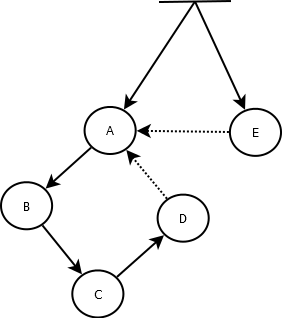
\includegraphics[width=0.32\textwidth]{figs/brownbridge}
	\caption{When root R deletes strong edge to A, through partial tracing A will have strong edge at the end.}
	\label{brownbridge}
\end{figure}

Figure ~\ref{brownbridge} shows an example graph where Brownbridge technique will identify the external support to a node and restores the graph. In figure ~\ref{brownbridge}, if strong edge to A is deleted, A will convert all incoming weak edges into strong and starts weakening the edges. When B receives weaken message, it weakens the edge and then converts all weak incoming edges to strong and weakens the edge to C. The process continues until it reaches A again. When the process reaches A, A realizes now it has additional strong incoming edge. So the graph is recovered now. If there is no edge from E to A, then the whole subgraph A, B, C an D will be deleted.


\section{Pitfalls of Brownbridge Garbage Collection}
The idea behind Brownbridge method is to identify external support for the node that lost the last strong incoming edge. If the external strong support to the subgraph comes to a node that is not the node that lost the strong incoming edge, then the method fails to identify them and prematurely delete nodes.  

\begin{figure}[!t]
\centering
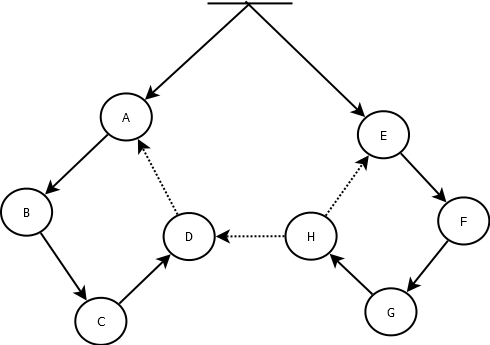
\includegraphics[width=0.47\textwidth]{figs/brownbridgefail}
\caption{When root R deletes strong edge to A, through partial tracing A will fail to identify liveness.}
\label{brownbridgefail}
\end{figure}

In figure ~\ref{brownbridgefail}, when root deletes edge to A, A starts partial tracing. When the partial tracing reaches back A, D has additional strong support. But algorithm only makes decision based on A's strong incoming edge. So the A, B, C, D subgraph will be deleted prematurely.


